\documentclass[tikz,border=10pt]{standalone}
\begin{document}
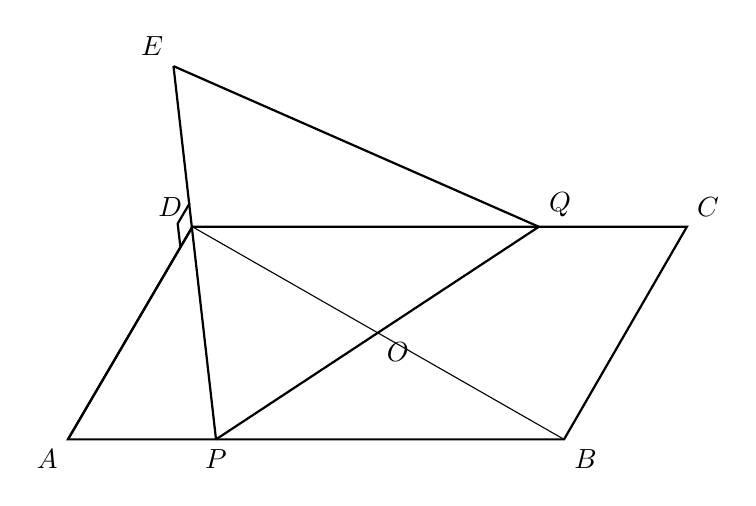
\begin{tikzpicture}[scale=1, line width=0.8pt]
  \coordinate (A) at (1.32,0);
  \coordinate (P) at (3.2,0);
  \coordinate (B) at (7.62,0);
  \coordinate (C) at (9.18,2.7);
  \coordinate (Q) at (7.3,2.7);
  \coordinate (D) at (2.9,2.7);
  \coordinate (E) at (2.66,4.74);
  \coordinate (O) at (5.24,1.36);

  \draw (A) -- (B) -- (C) -- (D) -- cycle;
  \draw (E) -- (Q);
  \draw (E) -- (P);
  \draw (P) -- (Q);
  \draw (A) -- (D);
  \draw[line width=0.4pt] (D) -- (B);

  \draw (2.748,2.441) -- (2.713,2.740) -- (2.865,2.999);

  \node[above left] at (E) {$E$};
  \node[above left] at (D) {$D$};
  \node[above right] at (Q) {$Q$};
  \node[above right] at (C) {$C$};
  \node[below right] at (O) {$O$};
  \node[below] at (P) {$P$};
  \node[below left] at (A) {$A$};
  \node[below right] at (B) {$B$};
\end{tikzpicture}
\end{document}
